% Options for packages loaded elsewhere
\PassOptionsToPackage{unicode}{hyperref}
\PassOptionsToPackage{hyphens}{url}
%
\documentclass[
]{article}
\usepackage{lmodern}
\usepackage{amssymb,amsmath}
\usepackage{ifxetex,ifluatex}
\ifnum 0\ifxetex 1\fi\ifluatex 1\fi=0 % if pdftex
  \usepackage[T1]{fontenc}
  \usepackage[utf8]{inputenc}
  \usepackage{textcomp} % provide euro and other symbols
\else % if luatex or xetex
  \usepackage{unicode-math}
  \defaultfontfeatures{Scale=MatchLowercase}
  \defaultfontfeatures[\rmfamily]{Ligatures=TeX,Scale=1}
\fi
% Use upquote if available, for straight quotes in verbatim environments
\IfFileExists{upquote.sty}{\usepackage{upquote}}{}
\IfFileExists{microtype.sty}{% use microtype if available
  \usepackage[]{microtype}
  \UseMicrotypeSet[protrusion]{basicmath} % disable protrusion for tt fonts
}{}
\makeatletter
\@ifundefined{KOMAClassName}{% if non-KOMA class
  \IfFileExists{parskip.sty}{%
    \usepackage{parskip}
  }{% else
    \setlength{\parindent}{0pt}
    \setlength{\parskip}{6pt plus 2pt minus 1pt}}
}{% if KOMA class
  \KOMAoptions{parskip=half}}
\makeatother
\usepackage{xcolor}
\IfFileExists{xurl.sty}{\usepackage{xurl}}{} % add URL line breaks if available
\IfFileExists{bookmark.sty}{\usepackage{bookmark}}{\usepackage{hyperref}}
\hypersetup{
  pdftitle={Course Project 1},
  hidelinks,
  pdfcreator={LaTeX via pandoc}}
\urlstyle{same} % disable monospaced font for URLs
\usepackage[margin=1in]{geometry}
\usepackage{color}
\usepackage{fancyvrb}
\newcommand{\VerbBar}{|}
\newcommand{\VERB}{\Verb[commandchars=\\\{\}]}
\DefineVerbatimEnvironment{Highlighting}{Verbatim}{commandchars=\\\{\}}
% Add ',fontsize=\small' for more characters per line
\usepackage{framed}
\definecolor{shadecolor}{RGB}{248,248,248}
\newenvironment{Shaded}{\begin{snugshade}}{\end{snugshade}}
\newcommand{\AlertTok}[1]{\textcolor[rgb]{0.94,0.16,0.16}{#1}}
\newcommand{\AnnotationTok}[1]{\textcolor[rgb]{0.56,0.35,0.01}{\textbf{\textit{#1}}}}
\newcommand{\AttributeTok}[1]{\textcolor[rgb]{0.77,0.63,0.00}{#1}}
\newcommand{\BaseNTok}[1]{\textcolor[rgb]{0.00,0.00,0.81}{#1}}
\newcommand{\BuiltInTok}[1]{#1}
\newcommand{\CharTok}[1]{\textcolor[rgb]{0.31,0.60,0.02}{#1}}
\newcommand{\CommentTok}[1]{\textcolor[rgb]{0.56,0.35,0.01}{\textit{#1}}}
\newcommand{\CommentVarTok}[1]{\textcolor[rgb]{0.56,0.35,0.01}{\textbf{\textit{#1}}}}
\newcommand{\ConstantTok}[1]{\textcolor[rgb]{0.00,0.00,0.00}{#1}}
\newcommand{\ControlFlowTok}[1]{\textcolor[rgb]{0.13,0.29,0.53}{\textbf{#1}}}
\newcommand{\DataTypeTok}[1]{\textcolor[rgb]{0.13,0.29,0.53}{#1}}
\newcommand{\DecValTok}[1]{\textcolor[rgb]{0.00,0.00,0.81}{#1}}
\newcommand{\DocumentationTok}[1]{\textcolor[rgb]{0.56,0.35,0.01}{\textbf{\textit{#1}}}}
\newcommand{\ErrorTok}[1]{\textcolor[rgb]{0.64,0.00,0.00}{\textbf{#1}}}
\newcommand{\ExtensionTok}[1]{#1}
\newcommand{\FloatTok}[1]{\textcolor[rgb]{0.00,0.00,0.81}{#1}}
\newcommand{\FunctionTok}[1]{\textcolor[rgb]{0.00,0.00,0.00}{#1}}
\newcommand{\ImportTok}[1]{#1}
\newcommand{\InformationTok}[1]{\textcolor[rgb]{0.56,0.35,0.01}{\textbf{\textit{#1}}}}
\newcommand{\KeywordTok}[1]{\textcolor[rgb]{0.13,0.29,0.53}{\textbf{#1}}}
\newcommand{\NormalTok}[1]{#1}
\newcommand{\OperatorTok}[1]{\textcolor[rgb]{0.81,0.36,0.00}{\textbf{#1}}}
\newcommand{\OtherTok}[1]{\textcolor[rgb]{0.56,0.35,0.01}{#1}}
\newcommand{\PreprocessorTok}[1]{\textcolor[rgb]{0.56,0.35,0.01}{\textit{#1}}}
\newcommand{\RegionMarkerTok}[1]{#1}
\newcommand{\SpecialCharTok}[1]{\textcolor[rgb]{0.00,0.00,0.00}{#1}}
\newcommand{\SpecialStringTok}[1]{\textcolor[rgb]{0.31,0.60,0.02}{#1}}
\newcommand{\StringTok}[1]{\textcolor[rgb]{0.31,0.60,0.02}{#1}}
\newcommand{\VariableTok}[1]{\textcolor[rgb]{0.00,0.00,0.00}{#1}}
\newcommand{\VerbatimStringTok}[1]{\textcolor[rgb]{0.31,0.60,0.02}{#1}}
\newcommand{\WarningTok}[1]{\textcolor[rgb]{0.56,0.35,0.01}{\textbf{\textit{#1}}}}
\usepackage{graphicx,grffile}
\makeatletter
\def\maxwidth{\ifdim\Gin@nat@width>\linewidth\linewidth\else\Gin@nat@width\fi}
\def\maxheight{\ifdim\Gin@nat@height>\textheight\textheight\else\Gin@nat@height\fi}
\makeatother
% Scale images if necessary, so that they will not overflow the page
% margins by default, and it is still possible to overwrite the defaults
% using explicit options in \includegraphics[width, height, ...]{}
\setkeys{Gin}{width=\maxwidth,height=\maxheight,keepaspectratio}
% Set default figure placement to htbp
\makeatletter
\def\fps@figure{htbp}
\makeatother
\setlength{\emergencystretch}{3em} % prevent overfull lines
\providecommand{\tightlist}{%
  \setlength{\itemsep}{0pt}\setlength{\parskip}{0pt}}
\setcounter{secnumdepth}{-\maxdimen} % remove section numbering

\title{Course Project 1}
\author{}
\date{\vspace{-2.5em}}

\begin{document}
\maketitle

\hypertarget{loading-and-preprocessing-the-data}{%
\subsection{1. Loading and preprocessing the
data}\label{loading-and-preprocessing-the-data}}

\begin{Shaded}
\begin{Highlighting}[]
\KeywordTok{library}\NormalTok{(data.table)}
\KeywordTok{library}\NormalTok{(tidyverse)}
\end{Highlighting}
\end{Shaded}

\begin{verbatim}
## -- Attaching packages --------------------------------------- tidyverse 1.3.0 --
\end{verbatim}

\begin{verbatim}
## v ggplot2 3.3.2     v purrr   0.3.4
## v tibble  3.0.4     v dplyr   1.0.2
## v tidyr   1.1.2     v stringr 1.4.0
## v readr   1.4.0     v forcats 0.5.0
\end{verbatim}

\begin{verbatim}
## -- Conflicts ------------------------------------------ tidyverse_conflicts() --
## x dplyr::between()   masks data.table::between()
## x dplyr::filter()    masks stats::filter()
## x dplyr::first()     masks data.table::first()
## x dplyr::lag()       masks stats::lag()
## x dplyr::last()      masks data.table::last()
## x purrr::transpose() masks data.table::transpose()
\end{verbatim}

\begin{Shaded}
\begin{Highlighting}[]
\NormalTok{path <-}\StringTok{ "/media/ad/01D6B57CFBE4DB20/1.Linux/Data/JHU data/activity.csv"}
\NormalTok{data <-}\StringTok{ }\KeywordTok{fread}\NormalTok{(path)}
\KeywordTok{head}\NormalTok{(data)}
\end{Highlighting}
\end{Shaded}

\begin{verbatim}
##    steps       date interval
## 1:    NA 2012-10-01        0
## 2:    NA 2012-10-01        5
## 3:    NA 2012-10-01       10
## 4:    NA 2012-10-01       15
## 5:    NA 2012-10-01       20
## 6:    NA 2012-10-01       25
\end{verbatim}

\begin{Shaded}
\begin{Highlighting}[]
\KeywordTok{tail}\NormalTok{(data)}
\end{Highlighting}
\end{Shaded}

\begin{verbatim}
##    steps       date interval
## 1:    NA 2012-11-30     2330
## 2:    NA 2012-11-30     2335
## 3:    NA 2012-11-30     2340
## 4:    NA 2012-11-30     2345
## 5:    NA 2012-11-30     2350
## 6:    NA 2012-11-30     2355
\end{verbatim}

The variables included in this dataset are:

\begin{itemize}
\tightlist
\item
  steps: Number of steps taking in a 5-minute interval (missing values
  are coded as NA)
\item
  date: The date on which the measurement was taken in YYYY-MM-DD format
\item
  interval: Identifier for the 5-minute interval in which measurement
  was taken
\end{itemize}

\hypertarget{data-exclude-na-value}{%
\subsection{2. Data exclude NA value}\label{data-exclude-na-value}}

\hypertarget{what-is-mean-total-number-of-steps-taken-per-da}{%
\subsubsection{2.1 What is mean total number of steps taken per
da}\label{what-is-mean-total-number-of-steps-taken-per-da}}

For this part of the assignment, you can ignore the missing values in
the dataset.

\begin{Shaded}
\begin{Highlighting}[]
\KeywordTok{dim}\NormalTok{(data)}
\end{Highlighting}
\end{Shaded}

\begin{verbatim}
## [1] 17568     3
\end{verbatim}

\begin{Shaded}
\begin{Highlighting}[]
\KeywordTok{sum}\NormalTok{(}\KeywordTok{is.na}\NormalTok{(data))}
\end{Highlighting}
\end{Shaded}

\begin{verbatim}
## [1] 2304
\end{verbatim}

\begin{Shaded}
\begin{Highlighting}[]
\NormalTok{null_value <-}\StringTok{ }\KeywordTok{sapply}\NormalTok{(data, }\ControlFlowTok{function}\NormalTok{(x) }\KeywordTok{sum}\NormalTok{(}\KeywordTok{is.na}\NormalTok{(x)))}
\NormalTok{null_value}
\end{Highlighting}
\end{Shaded}

\begin{verbatim}
##    steps     date interval 
##     2304        0        0
\end{verbatim}

\begin{Shaded}
\begin{Highlighting}[]
\NormalTok{data_exclude_na <-}\StringTok{ }\KeywordTok{na.omit}\NormalTok{(data)}
\KeywordTok{dim}\NormalTok{(data_exclude_na)}
\end{Highlighting}
\end{Shaded}

\begin{verbatim}
## [1] 15264     3
\end{verbatim}

\begin{Shaded}
\begin{Highlighting}[]
\NormalTok{step_per_day <-}\StringTok{ }\NormalTok{data_exclude_na[,.(}\DataTypeTok{total_step =} \KeywordTok{sum}\NormalTok{(steps)),by=date]}
\KeywordTok{head}\NormalTok{(step_per_day)}
\end{Highlighting}
\end{Shaded}

\begin{verbatim}
##          date total_step
## 1: 2012-10-02        126
## 2: 2012-10-03      11352
## 3: 2012-10-04      12116
## 4: 2012-10-05      13294
## 5: 2012-10-06      15420
## 6: 2012-10-07      11015
\end{verbatim}

\begin{Shaded}
\begin{Highlighting}[]
\CommentTok{#png("plot1.png", width=480, height=480)}
\NormalTok{step_per_day }\OperatorTok\StringTok{ }
\StringTok{  }\KeywordTok{ggplot}\NormalTok{(}\KeywordTok{aes}\NormalTok{(}\DataTypeTok{x=}\NormalTok{total_step))}\OperatorTok{+}
\StringTok{  }\KeywordTok{geom_histogram}\NormalTok{() }\OperatorTok{+}
\StringTok{  }\KeywordTok{labs}\NormalTok{(}\DataTypeTok{title =} \StringTok{"Histogram of total step per day"}\NormalTok{)}
\end{Highlighting}
\end{Shaded}

\begin{verbatim}
## `stat_bin()` using `bins = 30`. Pick better value with `binwidth`.
\end{verbatim}

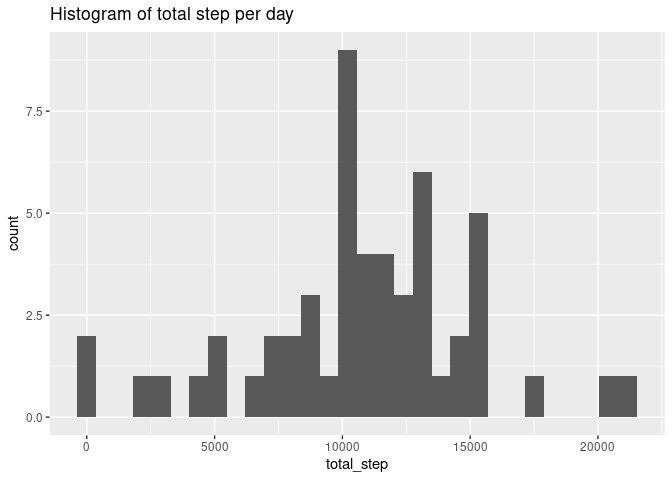
\includegraphics{PA1_template_files/figure-latex/unnamed-chunk-5-1.pdf}

\begin{Shaded}
\begin{Highlighting}[]
\CommentTok{# Method 1: mean and median by data.table function}
\NormalTok{step_per_day[,}\KeywordTok{c}\NormalTok{(}\KeywordTok{lapply}\NormalTok{(.SD,median),}\KeywordTok{lapply}\NormalTok{(.SD,mean)), .SDcols=}\StringTok{"total_step"}\NormalTok{]}
\end{Highlighting}
\end{Shaded}

\begin{verbatim}
##    total_step total_step
## 1:      10765   10766.19
\end{verbatim}

\begin{Shaded}
\begin{Highlighting}[]
\CommentTok{# Method 2: mean and median by summary function}
\KeywordTok{summary}\NormalTok{(step_per_day}\OperatorTok{$}\NormalTok{total_step) }
\end{Highlighting}
\end{Shaded}

\begin{verbatim}
##    Min. 1st Qu.  Median    Mean 3rd Qu.    Max. 
##      41    8841   10765   10766   13294   21194
\end{verbatim}

\begin{Shaded}
\begin{Highlighting}[]
\CommentTok{# median: 10765 , mean: 10766}
\end{Highlighting}
\end{Shaded}

\hypertarget{what-is-the-average-daily-activity-pattern}{%
\subsubsection{2.2 What is the average daily activity
pattern?}\label{what-is-the-average-daily-activity-pattern}}

Make a time series plot (i.e.~\color{red}{\verb|type = "l"|}type =
``l'') of the 5-minute interval (x-axis) and the average number of steps
taken, averaged across all days (y-axis)

\begin{Shaded}
\begin{Highlighting}[]
\NormalTok{average_steps_per_5min_interval <-}\StringTok{ }\NormalTok{data_exclude_na[,.(}\DataTypeTok{mean_step =} \KeywordTok{mean}\NormalTok{(steps)),by=interval]}
\KeywordTok{head}\NormalTok{(average_steps_per_5min_interval)}
\end{Highlighting}
\end{Shaded}

\begin{verbatim}
##    interval mean_step
## 1:        0 1.7169811
## 2:        5 0.3396226
## 3:       10 0.1320755
## 4:       15 0.1509434
## 5:       20 0.0754717
## 6:       25 2.0943396
\end{verbatim}

\begin{Shaded}
\begin{Highlighting}[]
\CommentTok{#png("plot2.png", width=480, height=480)}
\NormalTok{average_steps_per_5min_interval }\OperatorTok\StringTok{ }
\StringTok{  }\KeywordTok{ggplot}\NormalTok{(}\KeywordTok{aes}\NormalTok{(}\DataTypeTok{x=}\NormalTok{interval,}\DataTypeTok{y=}\NormalTok{mean_step)) }\OperatorTok{+}
\StringTok{  }\KeywordTok{geom_line}\NormalTok{()}
\end{Highlighting}
\end{Shaded}

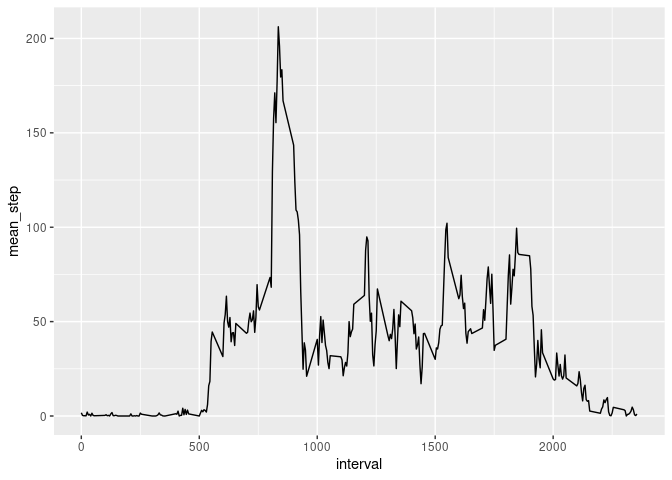
\includegraphics{PA1_template_files/figure-latex/unnamed-chunk-9-1.pdf}

Which 5-minute interval, on average across all the days in the dataset,
contains the maximum number of steps?

\begin{Shaded}
\begin{Highlighting}[]
\NormalTok{average_steps_per_5min_interval[}\KeywordTok{which.max}\NormalTok{(average_steps_per_5min_interval}\OperatorTok{$}\NormalTok{mean_step)]}
\end{Highlighting}
\end{Shaded}

\begin{verbatim}
##    interval mean_step
## 1:      835  206.1698
\end{verbatim}

\hypertarget{imputing-missing-values}{%
\subsection{3. Imputing missing values}\label{imputing-missing-values}}

\hypertarget{total-number-of-missing-values-in-dataset}{%
\subsubsection{3.1 Total number of missing values in
dataset}\label{total-number-of-missing-values-in-dataset}}

\begin{Shaded}
\begin{Highlighting}[]
\KeywordTok{sum}\NormalTok{(}\KeywordTok{is.na}\NormalTok{(data))}
\end{Highlighting}
\end{Shaded}

\begin{verbatim}
## [1] 2304
\end{verbatim}

\begin{Shaded}
\begin{Highlighting}[]
\CommentTok{# Find which column have missing value}
\KeywordTok{colSums}\NormalTok{(}\KeywordTok{is.na}\NormalTok{(data))}
\end{Highlighting}
\end{Shaded}

\begin{verbatim}
##    steps     date interval 
##     2304        0        0
\end{verbatim}

\hypertarget{devise-a-strategy-for-filling-in-all-of-the-missing-values-in-the-dataset.}{%
\subsubsection{3.2 Devise a strategy for filling in all of the missing
values in the
dataset.}\label{devise-a-strategy-for-filling-in-all-of-the-missing-values-in-the-dataset.}}

\begin{Shaded}
\begin{Highlighting}[]
\KeywordTok{summary}\NormalTok{(data}\OperatorTok{$}\NormalTok{steps,}\DataTypeTok{na.rm=}\OtherTok{TRUE}\NormalTok{)}
\end{Highlighting}
\end{Shaded}

\begin{verbatim}
##    Min. 1st Qu.  Median    Mean 3rd Qu.    Max.    NA's 
##    0.00    0.00    0.00   37.38   12.00  806.00    2304
\end{verbatim}

\begin{Shaded}
\begin{Highlighting}[]
\CommentTok{# impute with median value}
\NormalTok{data[}\KeywordTok{is.na}\NormalTok{(steps), }\StringTok{"steps"}\NormalTok{]  <-}\StringTok{ }\NormalTok{data[, }\KeywordTok{lapply}\NormalTok{(.SD, median, }\DataTypeTok{na.rm=}\OtherTok{TRUE}\NormalTok{), .SDcols =}\StringTok{ "steps"}\NormalTok{]}
\KeywordTok{head}\NormalTok{(data)}
\end{Highlighting}
\end{Shaded}

\begin{verbatim}
##    steps       date interval
## 1:     0 2012-10-01        0
## 2:     0 2012-10-01        5
## 3:     0 2012-10-01       10
## 4:     0 2012-10-01       15
## 5:     0 2012-10-01       20
## 6:     0 2012-10-01       25
\end{verbatim}

\hypertarget{create-a-new-dataset-that-is-equal-to-the-original-dataset-but-with-the-missing-data-filled-in.}{%
\subsubsection{3.3 Create a new dataset that is equal to the original
dataset but with the missing data filled
in.}\label{create-a-new-dataset-that-is-equal-to-the-original-dataset-but-with-the-missing-data-filled-in.}}

\begin{Shaded}
\begin{Highlighting}[]
\NormalTok{data.table}\OperatorTok{::}\KeywordTok{fwrite}\NormalTok{(}\DataTypeTok{x =}\NormalTok{ data, }\DataTypeTok{file =} \StringTok{"data_impute_median.csv"}\NormalTok{, }\DataTypeTok{quote =} \OtherTok{FALSE}\NormalTok{)}
\end{Highlighting}
\end{Shaded}

\hypertarget{make-a-histogram-of-the-total-number-of-steps-taken-each-day-and-calculate-and-report-the-mean-and-median-total-number-of-steps-taken-per-day}{%
\subsubsection{3.4 Make a histogram of the total number of steps taken
each day and Calculate and report the mean and median total number of
steps taken per
day}\label{make-a-histogram-of-the-total-number-of-steps-taken-each-day-and-calculate-and-report-the-mean-and-median-total-number-of-steps-taken-per-day}}

\begin{Shaded}
\begin{Highlighting}[]
\NormalTok{data <-}\StringTok{ }\KeywordTok{fread}\NormalTok{(}\StringTok{"data_impute_median.csv"}\NormalTok{)}
\KeywordTok{head}\NormalTok{(data)}
\end{Highlighting}
\end{Shaded}

\begin{verbatim}
##    steps       date interval
## 1:     0 2012-10-01        0
## 2:     0 2012-10-01        5
## 3:     0 2012-10-01       10
## 4:     0 2012-10-01       15
## 5:     0 2012-10-01       20
## 6:     0 2012-10-01       25
\end{verbatim}

\begin{Shaded}
\begin{Highlighting}[]
\NormalTok{step_per_day <-}\StringTok{ }\NormalTok{data[,.(}\DataTypeTok{total_step =} \KeywordTok{sum}\NormalTok{(steps)),by=date]}
\KeywordTok{head}\NormalTok{(step_per_day)}
\end{Highlighting}
\end{Shaded}

\begin{verbatim}
##          date total_step
## 1: 2012-10-01          0
## 2: 2012-10-02        126
## 3: 2012-10-03      11352
## 4: 2012-10-04      12116
## 5: 2012-10-05      13294
## 6: 2012-10-06      15420
\end{verbatim}

\begin{Shaded}
\begin{Highlighting}[]
\CommentTok{#png("plot3.png", width=480, height=480)}
\NormalTok{step_per_day }\OperatorTok\StringTok{ }
\StringTok{  }\KeywordTok{ggplot}\NormalTok{(}\KeywordTok{aes}\NormalTok{(}\DataTypeTok{x=}\NormalTok{total_step))}\OperatorTok{+}
\StringTok{  }\KeywordTok{geom_histogram}\NormalTok{() }\OperatorTok{+}
\StringTok{  }\KeywordTok{labs}\NormalTok{(}\DataTypeTok{title =} \StringTok{"Histogram of total step per day"}\NormalTok{)}
\end{Highlighting}
\end{Shaded}

\begin{verbatim}
## `stat_bin()` using `bins = 30`. Pick better value with `binwidth`.
\end{verbatim}

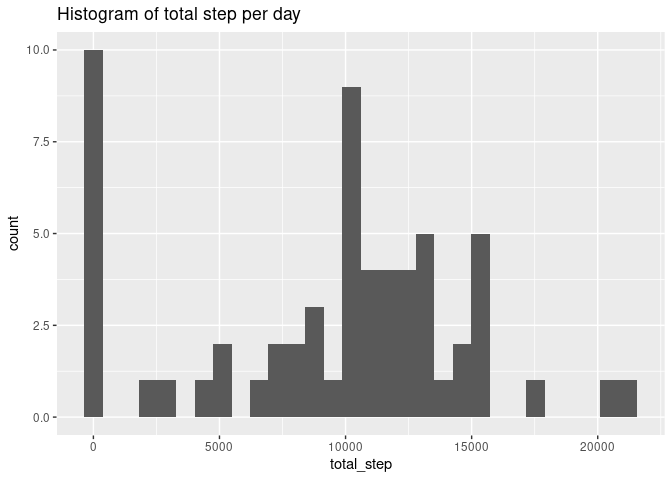
\includegraphics{PA1_template_files/figure-latex/unnamed-chunk-18-1.pdf}

\begin{Shaded}
\begin{Highlighting}[]
\KeywordTok{summary}\NormalTok{(step_per_day}\OperatorTok{$}\NormalTok{total_step) }
\end{Highlighting}
\end{Shaded}

\begin{verbatim}
##    Min. 1st Qu.  Median    Mean 3rd Qu.    Max. 
##       0    6778   10395    9354   12811   21194
\end{verbatim}

\begin{Shaded}
\begin{Highlighting}[]
\CommentTok{# data exclude na value: median: 10765 , mean: 10766}
\CommentTok{# data impute na value: median: 10395, mean: 9354}
\end{Highlighting}
\end{Shaded}

Impute value make median and mean lower than not impute value

\hypertarget{are-there-differences-in-activity-patterns-between-weekdays-and-weekends}{%
\subsubsection{3.5 Are there differences in activity patterns between
weekdays and
weekends?}\label{are-there-differences-in-activity-patterns-between-weekdays-and-weekends}}

\begin{Shaded}
\begin{Highlighting}[]
\NormalTok{data}
\end{Highlighting}
\end{Shaded}

\begin{verbatim}
##        steps       date interval
##     1:     0 2012-10-01        0
##     2:     0 2012-10-01        5
##     3:     0 2012-10-01       10
##     4:     0 2012-10-01       15
##     5:     0 2012-10-01       20
##    ---                          
## 17564:     0 2012-11-30     2335
## 17565:     0 2012-11-30     2340
## 17566:     0 2012-11-30     2345
## 17567:     0 2012-11-30     2350
## 17568:     0 2012-11-30     2355
\end{verbatim}

\begin{enumerate}
\def\labelenumi{\arabic{enumi}.}
\tightlist
\item
  Create a new factor variable in the dataset with two levels --
  ``weekday'' and ``weekend'' indicating whether a given date is a
  weekday or weekend day.
\end{enumerate}

\begin{Shaded}
\begin{Highlighting}[]
\KeywordTok{library}\NormalTok{(timeDate)}
\NormalTok{chec_weekend <-}\StringTok{ }\ControlFlowTok{function}\NormalTok{(date)\{}
  \ControlFlowTok{if}\NormalTok{ (}\KeywordTok{isWeekday}\NormalTok{(date,}\DataTypeTok{wday =} \DecValTok{1}\OperatorTok{:}\DecValTok{5}\NormalTok{))\{}
    \StringTok{"weekday"}
\NormalTok{  \}}
  \ControlFlowTok{else}\NormalTok{\{}
    \StringTok{"weekend"}
\NormalTok{  \}}
\NormalTok{\}}
\end{Highlighting}
\end{Shaded}

\begin{Shaded}
\begin{Highlighting}[]
\NormalTok{data[, week_day_check }\OperatorTok{:}\ErrorTok{=}\StringTok{ }\KeywordTok{mapply}\NormalTok{(chec_weekend, date)]}
\KeywordTok{head}\NormalTok{(data)}
\end{Highlighting}
\end{Shaded}

\begin{verbatim}
##    steps       date interval week_day_check
## 1:     0 2012-10-01        0        weekday
## 2:     0 2012-10-01        5        weekday
## 3:     0 2012-10-01       10        weekday
## 4:     0 2012-10-01       15        weekday
## 5:     0 2012-10-01       20        weekday
## 6:     0 2012-10-01       25        weekday
\end{verbatim}

\begin{enumerate}
\def\labelenumi{\arabic{enumi}.}
\setcounter{enumi}{1}
\tightlist
\item
  Make a panel plot containing a time series plot
  (i.e.~\color{red}{\verb|type = "l"|}type = ``l'') of the 5-minute
  interval (x-axis) and the average number of steps taken, averaged
  across all weekday days or weekend days (y-axis). See the README file
  in the GitHub repository to see an example of what this plot should
  look like using simulated data.
\end{enumerate}

\begin{Shaded}
\begin{Highlighting}[]
\NormalTok{mean_data <-}\StringTok{ }\KeywordTok{group_by}\NormalTok{(data, week_day_check, interval) }\OperatorTok
\StringTok{             }\KeywordTok{summarise}\NormalTok{(}\DataTypeTok{average_steps =} \KeywordTok{mean}\NormalTok{(steps))}
\end{Highlighting}
\end{Shaded}

\begin{verbatim}
## `summarise()` regrouping output by 'week_day_check' (override with `.groups` argument)
\end{verbatim}

\begin{Shaded}
\begin{Highlighting}[]
\KeywordTok{head}\NormalTok{(mean_data)}
\end{Highlighting}
\end{Shaded}

\begin{verbatim}
## # A tibble: 6 x 3
## # Groups:   week_day_check [1]
##   week_day_check interval average_steps
##   <chr>             <int>         <dbl>
## 1 weekday               0        2.02  
## 2 weekday               5        0.4   
## 3 weekday              10        0.156 
## 4 weekday              15        0.178 
## 5 weekday              20        0.0889
## 6 weekday              25        1.31
\end{verbatim}

\begin{Shaded}
\begin{Highlighting}[]
\CommentTok{#png("plot4.png", width=480, height=480)}
\NormalTok{mean_data }\OperatorTok\StringTok{ }
\StringTok{  }\KeywordTok{ggplot}\NormalTok{(}\KeywordTok{aes}\NormalTok{(}\DataTypeTok{x=}\NormalTok{interval,}\DataTypeTok{y=}\NormalTok{average_steps,}\DataTypeTok{colour =}\NormalTok{ week_day_check)) }\OperatorTok{+}
\StringTok{  }\KeywordTok{geom_line}\NormalTok{() }\OperatorTok{+}
\StringTok{  }\KeywordTok{facet_wrap}\NormalTok{(}\OperatorTok{~}\NormalTok{week_day_check)}
\end{Highlighting}
\end{Shaded}

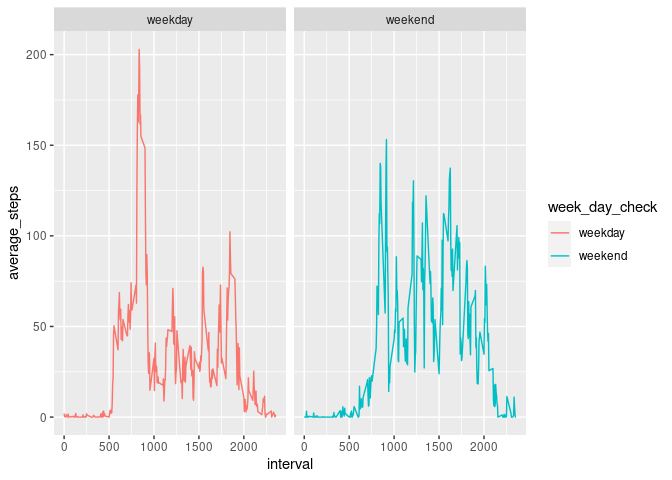
\includegraphics{PA1_template_files/figure-latex/unnamed-chunk-24-1.pdf}

\end{document}
